\documentclass[a4paper,11pt]{article}
\usepackage{verbatim,tocloft}
%--Add some fonts(probably unneccessary)
\usepackage{lmodern}
\usepackage[T1]{fontenc}
\usepackage{textcomp}
%--End
\renewcommand\cftsecfont{\normalfont}
\renewcommand\cftsecpagefont{\normalfont}
\renewcommand{\cftsecleader}{\cftdotfill{\cftsecdotsep}}
\renewcommand\cftsecdotsep{\cftdot}
\renewcommand\cftsubsecdotsep{\cftdot}
\usepackage{fourier-orns}
\usepackage{graphicx} % Need this for section 3.
\usepackage{makeidx,showidx} % For section 4.
% showidx package is useful for verifying the index.
\usepackage{fancyhdr}
\pagestyle{fancy}
\renewcommand{\sectionmark}[1]{%
\markboth{\thesection.\ #1}{}
}
\fancyhf{}
\fancyhf[HL]{\textsl{\leftmark}}
\fancyhf[HR]{\textsl{\rightmark}}
\fancyhf[FL]{\textbf{SON TO}}
\fancyhf[FR]{\thepage}
\renewcommand{\headrulewidth}{0.4pt}
\renewcommand{\footrulewidth}{0.4pt}
\renewcommand{\headrule}{\hrulefill
\raisebox{-2.1pt}[10pt][10pt]{\quad\decofourleft\decotwo%
\decofourright\quad}\hrulefill}
%\addtolength{\headheight}{\baselineskip}
%\renewcommand{\sectionmark}[1]{\markboth{#1}{}}
%\renewcommand{\subsectionmark}[1]{\markright{#1}}
%\rhead{\leftmark\\\rightmark}
\makeindex
\author{Son To $<$\href{mailto:son.trung.to@gmail.com}%
{son.trung.to@gmail.com}$>$}
\date{June 9th, 2016}
\title{Specialities}
\usepackage[pdftex,hyperindex=false,colorlinks=false,%
unicode]{hyperref}
% Or set links black, using \hypersetup{}
\begin{document}
  \maketitle
  \tableofcontents
  \newpage
  \section{Bibliograhy}
Partl~\cite{pa} has
proposed that \ldots
  \begin{thebibliography}{99}
    \bibitem[2]{pa}H.Partl:
    \emph{German \TeX},
    TUGboat Volume~9, Issue~1 (1988)
  \end{thebibliography}

\section{A lesson in Bib\emph{TeX}}
The next tutorial is taken from the
following link:
\bigbreak
\href{https://www.latex-tutorial.com/tutorials/beginners/latex-bibtex/}%
{BibTeX}
\flushleft
See Appendix.tex for the tutorial in Bib\emph{LaTeX}

The steps are:
\flushleft
\begin{enumerate}
  \item Create \verb+.bib+ file
  \item Following the sequence: La\TeX,Bib\TeX,La\TeX,La\TeX
\end{enumerate}
The result will be:
Random citation \cite{DUMMY:1} is embedded in the text.
\newpage
\bibliography{example}
\bibliographystyle{ieeetr}

\section{Including Encapsulated PostScript(.eps)}
driver=dvips, the most popular `dvi to POSTSCRIPT'
converter program, but this is sucked in PDF!

\begin{figure}[!htbp]
  \centering
  \fbox{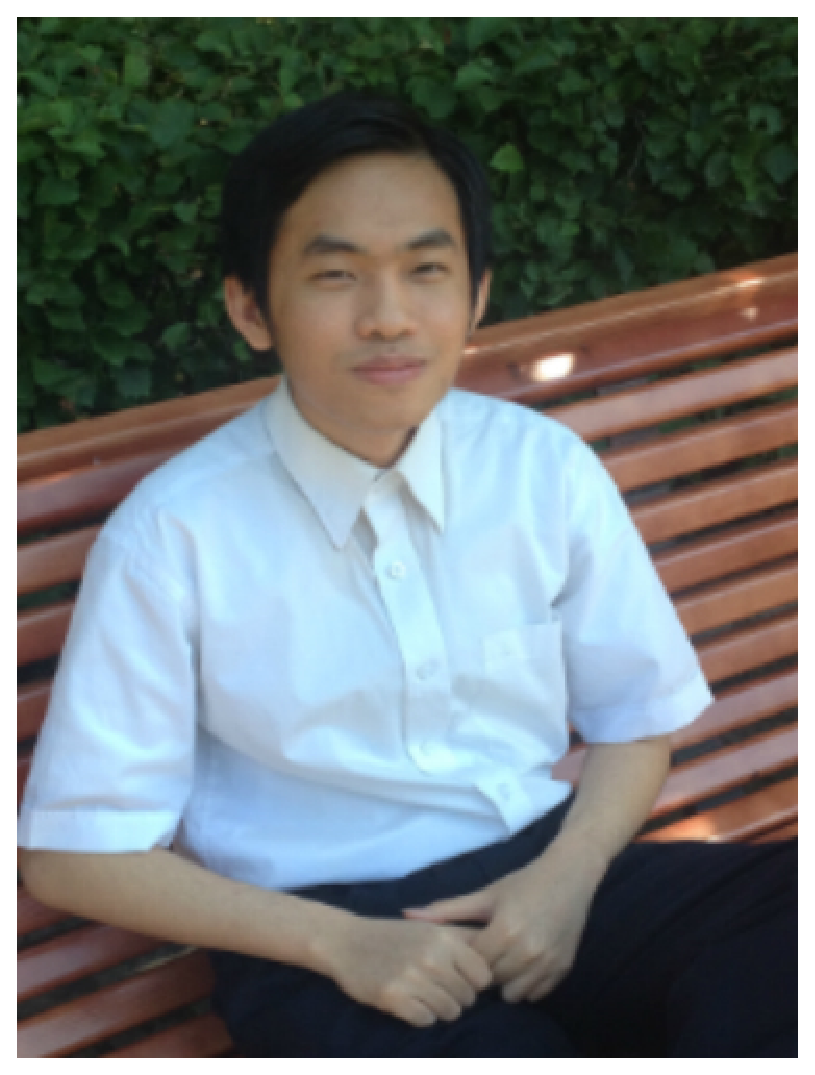
\includegraphics[scale=0.5]{picture2}}
  \caption{This is my picture}
  \label{}
\end{figure}

\section{Indexing}
Consider the following paragraph:
\paragraph{Gale-Shapley algorithm}
The Gale-Shapley
algorithm\index{Gale@\textbf{Gale-Shapley algorithm}}
forms a basic cornerstone for the study of two-sided
matching theory\index{match@\textsl{two-sided matching theory}},
one of the subfields of
game theory\index{game theory|textbf}.
\bigbreak
Remember to run
\begin{verbatim}
  makeindex filename
\end{verbatim}
to initiate the creation of \verb+.ind+ file, which contains the
sorted index and is processed by the input latex document.
\printindex

\section{Fancy Headers}
The default headers and footers in \LaTeX~are defined
by \verb+\pagestyle{}+ and \verb+\pagenumbering{}+

\section{\texorpdfstring{$E=mc^2$}{E=mc**2}}

\end{document}
